\documentclass[conference]{IEEEtran}
\IEEEoverridecommandlockouts
% The preceding line is only needed to identify funding in the first footnote. If that is unneeded, please comment it out.
\usepackage{cite}
\usepackage{amsmath,amssymb,amsfonts}
\usepackage{algorithmic}
\usepackage{graphicx}
\usepackage{textcomp}
\usepackage{xcolor}
\usepackage{enumitem}
\def\BibTeX{{\rm B\kern-.05em{\sc i\kern-.025em b}\kern-.08em
    T\kern-.1667em\lower.7ex\hbox{E}\kern-.125emX}}
\begin{document}

\title{Milestone 3: Dynamic Memory Optimization of Serverless Functions using RL/ML\\
{\footnotesize CS598 Cloud Computing Capstone Project (CCC) Fall 2023}
\thanks{University of Illinois, Urbana-Champaign.}
}

\author{\IEEEauthorblockN{Hao Zhang}
\IEEEauthorblockA{haoz18@illinois.edu}
\and
\IEEEauthorblockN{Yunxuan Li}
\IEEEauthorblockA{yunxuan6@illinois.edu}
\and
\IEEEauthorblockN{Cesar Arevalo}
\IEEEauthorblockA{cesara2@illinois.edu}
}

\maketitle

\section{Project Idea}
Our goal is to design and implement a framework that can automatically find and apply the optimal resource configuration for serverless functions in the fly, with the adoption of reinforcement learning algorithm (likely multi-armed bandit algorithm). The framework will support flexible and customizable optimization objective - minimal execution time, minimal cost, or a combination of the two. For a deployed FaaS function, the reinforcement learning agent would explore different configuration at the beginning, observe the feedback and reward in the fly, learn the pattern, and quickly converge to the optimal configuration choice. The framework should be capable of finding the optimal resource configuration for various types of FaaS functions. It should adapt to different workload patterns dynamically and quickly when input traffic starts to exhibit different behavior, which reflects the need of a new optimal config.

The framework is designed to support optimal memory configuration of AWS lambda function, but we believe this algorithm and workflow can be extended to other FaaS platforms as well.

\section{Justification}
Serverless computing has become a major paradigm of cloud computing, and the market is expected to maintain its growing trend in the upcoming future. When using FaaS (Function as a Service), users have to configure the memory size of their function \cite{aws-lambda}, \cite{10.1145/3429880.3430094}. While past research has shown that memory size of a FaaS function impacts its function performance greatly \cite{10.1145/3464298.3493398}, it is not trivial to identify the optimal memory configuration where function SLO (service level objective) is met and the cost is at the lowest \cite{9860980}. However, searching "memory optimization for FaaS/serverless function" in ACM digital library or IEEE Xplore does not yield many relevant results, indicating the potential of advancing research in this area. 

\subsection{Intellectual Merit}
The project explores the relationship between serverless function performance and variables such as function type, load size, request rate, in order to address the memory optimization problem encountered by FaaS users. It will help us better understand the potential benefits and downfalls of using both offline datasets and online in-prod data to train ML/RL models in order to control resource allocation of serverless functions. This research is intended to expand and deepen the understanding of dynamic FaaS memory optimization, and we expect it to help FaaS users to achieve easier and automated memory configuration that satisfies their expectation on execution time or cost.

\subsection{Novelty}
There has been previous research conducted to predict the cost of serverless function by mapping cloud resource configuration to local configuration via benchmark tool, then test application on local to find the resource needed and calculate cost \cite{9251165}. Previous research also studied different ways of optimizing serverless function/application for cost and performance. SLAM \cite{9860980} optimizes application (consist of serverless functions in DAG) execution time by measuring response time of each function and upgrade the resources allocated to the slowest function in iteration, until the end-to-end SLO is met. COSE \cite{10063937} uses Bayesian optimization and dynamically learn and update configuration until it converges, which can be used for both function-level and application-level optimization. To our best knowledge, there are no existing research that uses machine-learning or reinforcement learning algorithm, and takes function type, load size, request rate as input, to configure resource for serverless functions automatically and dynamically in response to change in workload and traffic patterns.

\subsection{Impact}
This project will contribute to the growing body of research on serverless computing, particularly in the area of resource optimization. The solution will demonstrate how resource allocation impacts serverless function performance, and more importantly, provide a painless solution to dynamic and automatic resource allocation of serverless functions. It has the potential to make serverless computing more affordable and practical, as well as increase the adoption of FaaS.


\section{Literature Survey}
\subsection{Resource Optimization for Serverless Functions}
Resource optimization in the serverless computing domain continues to be an area of active research and development \cite{10.1145/3587249, 10.1145/3406011, 9756233}, because of the constraints imposed to both the users and providers, i.e. memory, CPU, SLO/QoS, cost, scheduling, etc. \cite{10181224, 10.1145/3542929.3563469, 9860980, 9460548, 10.1145/3429880.3430099}. The resource optimization challenge can be categorized as follows, with solutions falling into a mix of these categories, as we will elaborate further:

\begin{enumerate}
    \item Perspective (of the): Users (e.g. FaaS developers); Providers (or FaaS platform)
    \item Use case: General (e.g. any function); application specific (i.e. DL training)
    \item Algorithm training: offline; online; or both
    \item Goal: Performance; cost
    \item Setup: Static (e.g. one-off, startup); Dynamic (e.g. during runtime)
\end{enumerate}

The FaaS Cloud Providers (e.g. AWS, GCP, Azure) are also doing research on resource optimization of their FaaS backends. Palette Load Balancing \cite{10.1145/3552326.3567496} utilizes locality hints for Serverless Functions on Azure, embedding locality as a firs-level concern in a FaaS platform for optimal performance and efficiency. AWS lambda is frequently updating it's service \cite{aws_new} and has sponsored research on cost/performance optimization \cite{aws_operating_lambda_performance_optimization}.

FaaS framework research includes Kraken \cite{10.1145/3472883.3486992}, focused on the optimization of container scheduling and provisioning for FaaS in a container environment, while meeting SLOs. Hermod \cite{10.1145/3542929.3563468} researched the optimal scheduling or serverless functions, built on Apache OpenWhisk, it demonstrated significant performance improvements on slowdown and load. Cypress \cite{10.1145/3542929.3563464} developed an algorithm for serverless platforms that handles container provisioning and request scheduling while being input size-sensitive. Manner et al \cite{9860370} compared commercial and open-source FaaS platforms resource optimization, providing insights into the QoS scaling of resources, providing different outcomes with regards to the linear scaling of performance vs costs.

From a FaaS user perspective, the COSE \cite{9155363} framework uses Bayesian Optimization to find the optimal configuration of serverless functions, and it uses statistical learning techniques to predict cost and execution times. Ali et al. \cite{10063937} continued the work on COSE, furthering the research on the use of Bayesian optimization of configuration parameters, with the goals of adhering to SLO requirements and optimizing for cost. However, these solutions do not perform as well under varying input sizes, and there is an overhead to the sampling data required to update the dynamic function parameters. To the best of our knowledge, we are now aware of any previous researches utilizing multi-armed bandit, or more generally, reinforcement learning algorithms to address resource optimization issues of FaaS functions. 

Research has been done on different FaaS use cases, eg. single-function \cite{10.1145/3429880.3430099, 9946331, 9881584}, multi-functions applications \cite{s23187829, 8567674} or application specific \cite{9826021} (eg. Deep learning training). Sizeless \cite{10.1145/3464298.3493398} predicts the optimal size of a single function, using synthetic data and production monitoring data to train an NN model (offline), with the objective function a mix of cost and execution time, allowing for a flexible trade-off. Costless \cite {8567674} optimizes for both cost and execution time of multiple functions, idenfitying when multiple functions could be fused into one, systematically deciding on which functions to fuse, and determining an optimal memory allocation for each function. SLAM \cite{9860980} is a tool that optimizes memory of multiple-functions depending on their SLO requirements, and other user-defined goals like minimizing cost or increasing performance. Astra \cite{9460548} automatically orchestrates and configures serverless analytics jobs (eg. map/reduce) while taking into account flexibly-specified user requirements (eg. performance, cost) and multi-dimensional factors (e.g., function memory size, degree of parallelism at each stage), leveraging graph theory (eg. Djikstra's and DAGs) it finds the optimal job execution, optimizing for either cost and/or time.

The offline resource optimization algorithms have required either training datasets \cite{10.1145/3464298.3493398, 10.1145/3542929.3563468}, the pre-processing of lambda functions for setup \cite{10.1109/INFOCOM48880.2022.9796962, 8567674}, sampling of functions to obtain profile metrics \cite{10.1145/3542929.3563464}, or function introspection to gauge resource utilization \cite{s23187829, 9336272}. All of these approaches have drawbacks, they either require overhead in time spent obtaining the datasets, have costs incurred on running the sampling functions, or they are using synthetic/artificially generated application metrics.

The online approaches for resource optimizations have used various ways to gather performance metrics (e.g. memory, CPU, etc.). The use of log parsing has been broadly used in cloud providers (eg. AWS Lambda), to drive algorithms whose outputs drive the reconfiguration of functions \cite{10063937, 9860980}. Similarly, research on FaaS frameworks, e.g. OpenWhisk, OpenFaaS, has been able to leverage a combination of monitoring tools, orchestrator/scheduler logs, and underlying architectures for gathering performance metrics \cite{9582234, 10.1145/3472883.3486992, 9946331}. However, these approaches require significant setup time for obtaining the performance metrics, or they are not used in a dynamic manner to reconfigure the functions automatically.

Ginzburg et al \cite{10.1145/3429880.3430099} demonstrated that the AWS Lambda performance variability is significant, and it is stable enough to exploit, with the conclusion that further optimizations by the cloud provider are still needed. The solutions proposed included delaying and/or scheduling workloads at various times, something that can be impractical for latency critical workloads.

The Lambda Power Tuning Tool by AWS \cite{aws_lambda_power_tuning} has the capability to optimize for either cost or execution time, but it requires a minimum of requests to be made against the lambda function, which can be cost prohibitive or impractical. Our system aims to streamline the tuning process and not require it to run the function a lot of times before being able the optimization happens.

\subsection{Online Learning: Reinforcement Learning and Multi-Armed Bandit}
\subsubsection{Reinforcement Learning}

Reinforcement learning refers to having an agent learn to pick the optimal behavior given a dynamic environment in order to maximize an objective. An agent selects an action and send it to an environment, based on observed historical data. The agent then observes reward from the environment on the selected action, and updates itself given the feedback. This process keeps iterating until some criteria is met. 

A typical reinforcement learning algorithm consists of these main components: 
\begin{itemize}
    \item Environment, which is the scenario in which the agent operates
    \item Reward/Cost. This is the observed objective returned by the environment. The goal of the algorithm is usually to maximize the cumulative reward, or minimize the cumulative cost.
    \item State. The current state of the environment. Here the assumption the environment could change over time.
    \item Policy. This is the method an agent use to determine which action to take, given input information.
\end{itemize}

In each trial, the reinforcement learning agent decides the action to be applied on the environment, and observes the corresponding feedback of that selected action.

\subsubsection{Multi-Armed Bandit}

Multi-armed bandit (MAB) is a simplified version of reinforcement learning algorithm, where environment is stateless, so the agent only needs to learn about the user behavior and the corresponding reward in order to pick one arm from all candidate arms to maximize the desired reward. An arm here refers to one of the candidate actions an agent can take. Exploration and exploitation are two key concepts here: exploration refers to the agent picks a suboptimal action, and learns from the feedback to shift away from choosing it in future; exploitation refers to the behavior of choosing the known optimal arms in order to maximize reward. The trade-off between exploration and exploitation is the central problem MAB algorithms try to tackle.

Popular MAB algorithms include Thompson Sampling, which explores and exploits given posterior distribution of rewards. It was evaluated Chapelle and Li\cite{NIPS2011_e53a0a29} and showed state-of-the-art level of performance. Other algorithms include Upper Confidence Bound(UCB), which chooses the action with highest upper confidence bound of predicted reward, and Epsilon-Greedy, which randomly chooses one arm with a probability of \(\alpha\), and chooses the best action with \((1-\alpha)\) probability.

\subsubsection{Contextual Multi-armed Bandit}

Vanilla MAB algorithms only use observed reward to find the optimal arm. However, in certain circumstances, other context of the trial could also influence which arm would lead to the optimal reward. These extra information additional to the reward metric are called contextual features. 

Bietti et al. \cite{10.5555/3546258.3546391} provides a systematic overview of how multi-armed bandit optimizes for a given reward using contextual features. Generally speaking, adopting contextual features in MAB involves training a machine learning model inside the MAB agent to predict reward given input features, and then add a layer of explore/exploit strategy on top of the model prediction to generate recommendations. 

We believe this Contextual Mult-armed Bandit idea could be further expanded to optimize for resource configuration for FaaS functions given different features of incoming requests, because different kinds of requests could lead to varying execution times, so incorporating these extra information as contextual features could optimize the resource allocation efficiency.
\vspace{12pt}

\section{System Architecture and Implementation}

\begin{figure*}
    \centering
    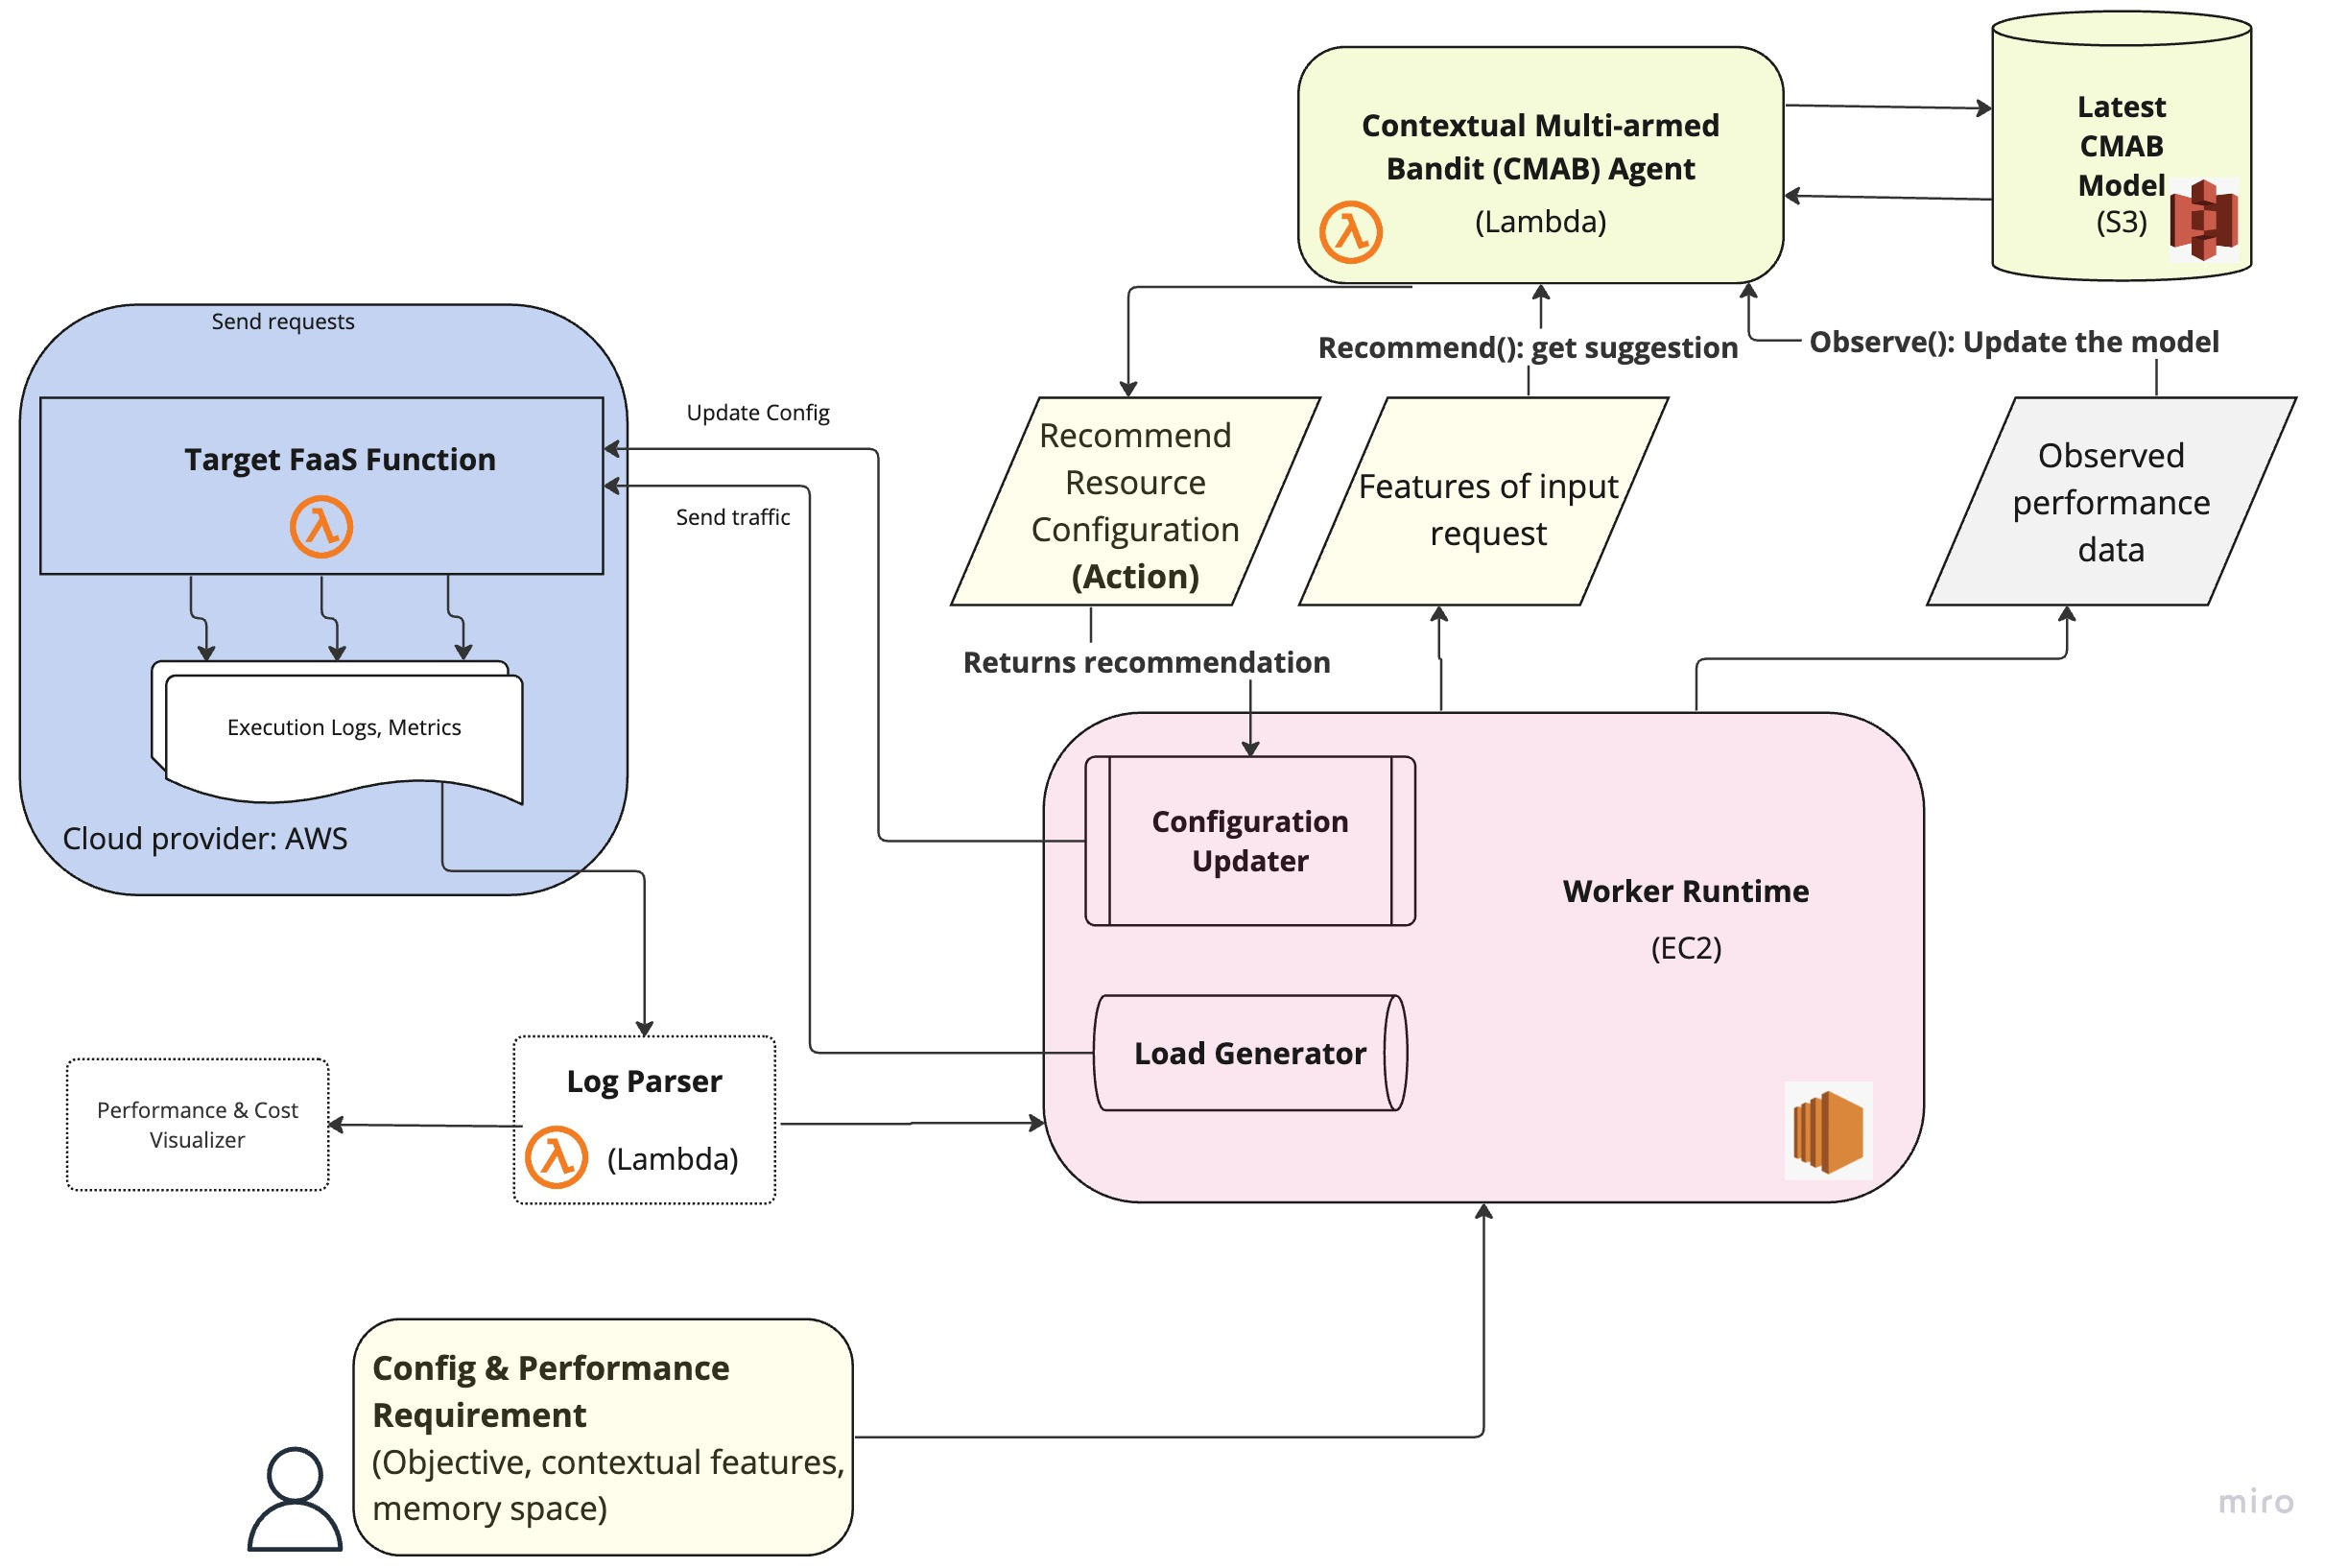
\includegraphics[width=1\linewidth]{System Architecture New.PNG}
    \caption{High-level architecture of the system and the interaction
between its components in a general use case}
    \label{fig:enter-label}
\end{figure*}

The latest high-level overview of the system workflow can be found in Figure 1. We implemented our system on Amazon Web Services (AWS), but this framework could easily be expanded to other cloud providers. Our code is available in a github repo (private) \footnote{https://github.com/yunxuanuiuc/Dynamic\_FaaS\_Resource\_Optimization}. 

The framework consists of the following components:
\begin{itemize}


\item CMAB-based Reinforcement Learning Agent (implemented).

The core of the system is a contextual multi-armed bandit (CMAB) agent, a type of reinforcement learning algorithms, which observes historical performance data of the target FaaS function, and makes recommendation on the ideal memory size for the same FaaS function. 

The algorithm is implemented using VowpalWabbit \cite{vowpal-wabbit}, an open-source contextual bandit package that supports easy integration of basic CMAB algorithms. The CMAB agent lives in a separate lambda function to support flexible memory optimization request at any time. Because of the stateless nature of lambda functions, we use AWS S3 to store the learned model, and load it to the CMAB agent lambda function when it is triggered.

The CMAB agent requires the basic information of the optimization problem to be set up. We need to pass in the follow information: 
\begin{itemize}
    \item The objective, i.e., the reward to optimize for. Per our problem statement, it supports either "time" or "reward" as objective.
    \item A list of candidate memory sizes. In AWS, the only configurable resource of FaaS functions is memory. Note that here we narrow down the search from a continuous memory space to a finite set of memory candidates for more efficient search. These memory sizes will be explored and the agent will learn to find the optimal candidate among them.
    \item A list of contextual features. These are the features of the requests that the target function receives, e.g, number of bytes of an input request.
    \item Model name. This is the name of the model, which will be used to save/load the CMAB model file.
    \item Model path. This is the place in local storage of the agent lambda function where the CMAB model will be downloaded from S3, or be written to after the CMAB model state is updated before being uploaded to S3.
\end{itemize}

This CMAB agent supports two types of APIs. In either of the following cases, we need to pass in S3 bucket and key data, in addition to the above parameters in order to initialize the CMAB model before loading a model file if there exists one. The agent will check if there is an existing model in the S3 bucket, and load it to the agent. Otherwise it will initialize a new model without historical learning.
\begin{enumerate}
    \item Observe. This API takes the actual memory size, probability of selecting that memory size, the observed reward, and the contextual features of a historical request of a FaaS function, and update the model parameters of the CMAB model. The updated model will be uploaded to S3.
    \item Recommend. This API takes the contextual features of a incoming request, and returns the (suggested memory size, probability of suggested memory size) tuple, which will be used for the memory config to update the memory configuration of the target lambda function.
\end{enumerate}

\item Logs Processor (implemented).

The Logs Processor ingests new logs produced by the Lambda function, and uses regular expression to extract useful data that will be used by the RL agent to model the function performance. These data include overall function execution time, memory usage, maximum memory configured, size of the incoming request that the function receives and function type. Among them, the first three are logged by Lambda and does not need additional logging. The latter two (input size and function type) needs custom logging in the lambda function. The parsed data will also be stored to database, and later be consumed by Performance and Cost Visualizer (to be developed) that allows us to monitor the agent's performance. 

The Logs Processor runs in an independent Lambda function and subscribes to log streams of the tested functions. Subscription filters are setup to select desired logs and feed the stream to Logs Processor.

\item Configuration Updater (implemented)

The Config Updater takes a FaaS function and a desired memory size as input, which comes from the CMAB agent. It then updates the memory configuration of the designated FaaS function, using AWS CLI. The script has been implemented, and it will be added as part of Worker Runtime for easier collaboration with other components.

\item Load Generator (implemented)

The Load generator is a program that can make requests to different target FaaS functions, this will allow us to explore the performance of FaaS functions under different memory settings. It can run with various configurations and/or runtime parameters:
\begin{itemize}
    \item workload: the type of function to run, the load generator can currently support two types of workloads - low-workload or high-workloads.
    \item duration: the amount of time in seconds that the program should run for.
    \item wait period: the amount of time to wait between sending requests to the lambda function.
\end{itemize}

Making different patterns of requests is yet to be developed, eg. not just a wait duration but maybe a random duration or at specific schedules, etc.

The actual function/application we plan to test are listed in Table 1, following the classification of FaaS functions developed by Zhang et al. \cite{10.1007/978-3-030-96326-2_2}. Experimenting on these four functions of different type should provide a comprehensive view of how practical is our system in different area of applications.

We plan to add the Load Generator to the same Virtual Machine the Worker Runtime lives in, for easier collaboration.


\item System (Worker) Runtime (to be implemented)

This is the main difference between this design and the original workflow. We realized we needed a central platform to connect different components after implementing all those components, and then decided to use a Worker Runtime to fulfill these tasks. This is yet to be implemented, but will be done shortly on a AWS EC2 Virtual Machine (VM).

The Worker Runtime will be the central component that drives the entire workflow, interacts with different components to accomplish the overall objective to update memory configuration dynamically. 

It will perform the following tasks, which also shows how the system works collectively:
\begin{enumerate}
\item Schedule the Load Generator to generate requests traffic with specific patterns to the target FaaS function. The FaaS function will execute and emit logs, which will trigger the Logs Processor to parse logs.
\item Get the parsed metrics from Logs Processor for each FaaS execution. Wrap the observed metrics and context features for each FaaS execution
\item Communicate with CMAB agent to observe the new performance data, via the agent's Observe() method.
\item Communicate with CMAB agent to get latest recommendation on the optimal memory size. Periodically takes an input request, get the conext features and send that to CMAB agent via the agent's Recommend() method.
\item Trigger the Configuration Updater to update the memory size of the target FaaS function, after getting the recommended memory size from the CMAB agent.

\end{enumerate}

\end{itemize}

\begin{table*}
\centering

\begin{tabular}{| l | l | l |}
\hline
Category & Description & Language \\
\hline

\hline
CPU-intensive function & Compute complex mathematical formulas using multiple threads & Python \\
\hline
Memory-intensive function & Summation of large integer arrays & Java \\
\hline
Image processing application & Image recognition & Java \\
\hline
Big data processing function & Word frequency statistics & Python \\
\hline

\end{tabular}
\caption{Four functions to Deploy and Test}
\label{table: 1}
\end{table*}


\section{Experiment setup description}
At this point, we implemented all individual components except for the worker runtime, just finished unit testing each of the components, and is in the process of integrating them into one unified system via worker runtime. We have not run large-scale tests to validate our hypotheses, but plan to start that very soon. 
\subsection{What hypothesis do you want to test?}
We would like to test three hypotheses.
\begin{itemize}
\item For a given FaaS function, the proposed framework is able to find out the optimal memory configuration quickly under stable workload.

Similarly, we will test both time to convergence and accuracy of our system, by sending stable workload to FaaS functions. We plan to compare the performance with a baseline method, Sizeless \cite{10.1145/3464298.3493398}, to show our method is more efficient in finding an optimal memory value.


\item With the adoption of this system, FaaS executions should comply with SLO requirements, and are able to achieve optimal/near-optimal objective.

We will implement a few types of FaaS applications, apply our framework, specify different SLO requirements, and generate synthetic traffic to the lambda functions in order to measure how well do these functions adhere to specified SLO, as an indicator of the effectiveness of our system.

\item When the incoming workload changes, the proposed framework would quickly detect and react by dynamically updating the optimal memory configuration, in order to ensure adherence to SLO and other objectives.
We will send requests with different sizes to the functions at different frequency, and understand how our system adjusts the recommended memory in response to varying traffic volume.
\end{itemize}

\subsection{What measurements do you intend to collect? Why \& What for?}

We plan to measure the performance of the proposed framework using a few synthetic/real-world FaaS functions. Functions would each represent a different type of common applications, for instance, network-intensive task or CPU-intensive task. We will evaluate the performance independently for each of the chosen FaaS functions. 

For each FaaS function, it will first be set up in AWS Lambda. The traffic generator will send out synthetic requests that follow a specified pattern. The proposed framework will be implemented and configured to oversee this target FaaS function. 

First, without the interference from the optimization framework, the execution time and associated cost of synthetic requests will be measured at different memory sizes. This will be used as baseline data to identify the optimal memory size given user specified optimization goal.

Then, we will turn on the optimization framework and let it optimize the memory configuration of the target lambda function in the fly. Again, the execution time and associated cost of each of the requests will be measured, as well as the memory size that is suggested by the framework in each round. We will also track the sequence of the requests in order to monitor convergence.

For each of the three hypotheses, there will be slight differences in the system setup as well as the metrics to compare:

\begin{itemize}
\item The ability to find out the optimal memory size under stable traffic patterns, given different optimization objectives (e.g., execution time or budget).

For this hypothesis, synthetic traffic will have similar input sizes in relatively steady pace, mimicking the scenario where a service receives stable and similar requests coming in throughout the day. 

From the baseline data, we will be able to pick the optimal/suboptimal memory size, which serves as the ground truth. We then compare the final memory size that the system converges to with the ground truth, and measure how well does the system successfully find the actual optimal/sub-optimal memory sizes for each FaaS function. Specifically, we plan to measure the percentage of times the system finds the optimal memory size, as well as number of rounds it takes the system to reach a stable memory size recommendation.

\item Compliance to SLO while optimizing for other objectives.

For this hypothesis, the system setup would be the same as the previous scenario. The execution time of each request will be compared against the SLO to understand how well this system is able to comply to SLO requirement.

Given other objectives, e.g., cost, we will also collect cost for each request, and measure against baseline cost to understand the system's ability to optimize cost while adhering to SLO.


\item The ability to dynamically determine optimal memory configuration given changing request patterns.

Synthetic requests sent out by the traffic modeler will be configured to have very different patterns throughout the day, categorized into several cohorts. For instance, one cohort would have a large size of requests, potentially demanding a lambda with higher memory size to support it, while another cohort would consist of lightweight requests. 

Again, we start with collecting baseline data, i.e., execution time and cost at different memory sizes, without interference of the optimization framework. This gives us the optimal memory size for each cohort.

We then turn on optimization framework. For each cohort, we plan to measure execution time, cost, and memory size it picks for each request. We will look at the data and identify the final memory size the algorithm converges to for each cohort, and compare to the ground truth to see if the algorithm picks the right memory size dynamically for different cohorts.

Additionally, we will measure the number of rounds it takes for the algorithm to converge to the new optimal point, which demonstrates how fast it is able to adapt to traffic change.

We will also measure the percentage of requests that confirm to SLO in this scenario, as an extra piece of evidence of the SLO adherence.

\end{itemize}


\subsection{What will a successful outcome look like?}
For each of the three hypotheses, a successful outcome should look like:
\begin{itemize}
%TODOTODOTODO
\item The ability to find out the optimal memory size under stable traffic patterns, given different optimization objectives (e.g., execution time or budget).

In this experiment, we expect to see that the converged memory size proposed by the framework is the same as the actual optimal memory size from the ground truth data, for all FaaS functions that we test. Additionally, we expect to see that it only takes a small number of iterations of memory configs before the algorithm makes a convergence, indicating that the algorithm is able to quickly find the optimum.

\item Compliance to SLO, while optimizing for other objectives.

The first experiment looks at how well the algorithm optimizes for a given objective. In this experiment, we want to validate that the algorithm is able to adhere to the specified SLO. We expect to see that with the proposed optimization framework, there is a high percentage of requests with execution times below SLO threshold. 

\item The ability to dynamically determine optimal memory configuration given changing request patterns.

We expect to see that once the pattern of input requests changes, the algorithm takes only a small number of requests to find out the new optimal memory size. This reflects how quickly the algorithm is able to dynamically find optimal memory configurations. Throughout the experiment, we also expect to see a high percentage of requests conforming to SLO while the pattern of input requests changes once in a while.

\end{itemize}

\section{Discussion}

\subsection{Challenges \& Future Optimization Opportunities}
We encountered a couple of challenges when starting to implement the system.

The VowpalWabbit-based CMAB model can only be stored and loaded using the built-in methods of VowpalWabbit workspace. However, the built-in methods to save and load the model only accept filepaths from the standard filesystem, meaning that in the CMAB agent lambda function, we cannot load model from S3 bucket directly using S3 filepath as it is not part of the standard filesystem. VowpalWabbit models also do not support serialization like what pickle would do. We came up with a workaround to use the temporary storage of CMAB agent lambda as a intermediate layer to communicate with S3 and the read/write methods of VowpalWabbit workspace separately, as filepaths in lambda storage are actually considered as standard. This is doable when the model size is small, but may become a problem if the model keeps growing. 

While lambda function is flexible and easy to use, it actually introduces some latency concerns, as the stateless lambda function needs to download and upload the model to S3 every time it is triggered. One potential optimization is to migrate the CMAB agent to a Virtual Machine (VM), spin it up as a service/daemon. This way, the agent does not need to reload the previously trained model every time, and there is also enough space to store the model. We do need to think of the cost of keeping a VM in this case.

There is also opportunities to optimize the CMAB agent algorithm. For the current MVP implementation, the agent treats all data equivalently, which may lead to slow reaction to dynamic input patterns changes. We will explore tuning the hyperparameters\cite{vw_parameters} such as learning rate and decay factor in order to improve model performance. If there is enough time, we can consider doing feature selection to find and use the most important features that contribute to time and cost estimation.

Several implementation options for Logs Processor are available. We first tried using a lambda function that runs in maximum time span (15mins) and queries for new log in a loop. This approach had significant drawbacks, as it's inefficient (running while the tested function is inactive) and it's hard to determine when to be triggered. The current approach, where Logs Processor is also a lambda function, but subscribes to and triggered by filtered log streams, is much more efficient. However, We've yet to find out the cost of feeding log streams and running the Logs Processor.

For storage and visualization of execution data, we considered threee database options: Aurora (MySQL), MongoDB (NoSQL), and Timestream. Timestream is a time-series database service that can handle large scale, high velocity data. Although it does seem to fit our requirement, Timestream is set aside for now as we do not have time to learn this new technology. It also a unknown if there is open-source equivalent of Timestream, that if ever needed, the system can migrate to. We'll use Aurora as of now, as execution data are structured and the number of records should remain in less than 10K.

Last but not least, the following design and the implementation question of the worker runtime still need to be discussed and outlined. 1. How does it decide when to call the RL Agent for recommendation? Is it based on the observed performance, or fixed interval? 2. How does it receive data from Log Processor (maybe an API endpoint)? What does it do with the data other than forward it to RL Agent? The forwarding can be skipped as it's easy to call RL Agent (lives in a Lambda function) from Logs Processor (another Lambda function. 3. It is planned to train the RL agent so that it can handle different types of function. Does the worker runtime need to orchestrate multiple synthetic function?

\subsection{Next steps}
% Yunxuan's thoughts: 
% implement the rest missing components
%% worker runtime (centralized place which initializes load generator, receives logs, interact with cmab agent)
%% deploy load geenrator() (i assume it's not deployed on AWS yet)
%% config updator
% test on 3 experiments
% refine the components (e.g., support easier configuration of cmab agent)
% improve cmab agent algorithm
% open question - now we only optimize for cost/time. Do we need some way to take SLO into account? or should we pivot if there is no time? 

These are the next steps tasks:

\subsubsection{System (worker) runtime}

The System (worker) runtime is still pending to be implemented, from our initial design to our current design, we realized that we needed a runtime for the configuration updater, the load generator, and (potentially) the Logs Processor.

We are planning on implementing this system on one or multiple VMs in AWS, using either EC2, Fargate, or EKS. The requirements here are to have a long-running system that can allow us to run one or more of the various components, either at different times or in conjunction (in parallel). This system needs to be setup with python library dependencies for our python codebase, and also have the right security configurations for communicating with the lambda functions, S3, and any database we may be using.

The modules we are planning on running as part of this system are: (a) Configuration Updates; (b) Load Generator; (c) Logs Processor (if needed); (d) Performance and Cost Visualizer.

\subsubsection{Logs Processor and CMAB integration}

The Logs Processor to CMAB agent integration requires the implementation of the outputs from the Logs Processor to be consumed by the CMAB agent, utilizing the System Runtime as the intermediate platform.

The Logs Processor needs to pass the extracted data to the CMAB agent, we are planning on using direct lambda call implementations. The CMAB agent is meant to act upon the data passed into it, perform an observation and potentially make a recommendation.

Another part of the Logs processor that is pending implementation is the saving of the extracted data to the database, for further analysis and/or visualization. We are planning on using the data from the database for the Performance and Cost Visualizer tool.

\subsubsection{Synthetic Functions and Load Generator}

The synthetic functions for the four different types of workloads need to be finalized, setup and made available as configurable workloads from the load generator.

The four functions we are planning on using for our experiments are (1) CPU-intensive function (Python), (2) Memory-intensive function (Java), (3) Image processing application (Java), and (4) Big data processing function (Python). The coding for the functions is pending.

For each of the functions developed, we need to have them setup as an AWS Lambda function, and these functions need to be configured from the load generator. Once they are configured, then the load generator can make requests to these functions at runtime.

The load generator at runtime can be configured to make requests to the different configured lambda functions, with configurations to simulate different workloads, low-workloads and high-workloads, with variable runtime durations for the load generator.

The load generator will allow us to gather training data for the CMAB agent, and test the dynamic configuration update capabilities of the system.

\subsubsection{Config Updater}

Configuration updater module is still a WIP, we need to hook it up from the outputs of the CMAB agent, and implement the capability for the update of the FaaS functions.

The configuration updater needs to integrate with the CMAB agent, to read the configuration updates recommended by the CMAB agent. These recommendation updates need to then be passed onto the Target FaaS function at runtime to change their settings, this is done at runtime using the AWS API (Python).

\subsubsection{Benchmarking}

Baseline method comparison, Sizeless \cite{10.1145/3464298.3493398}, needs to be implemented, setup, run and outputs gathered for the purpose of benchmarking.

If needed, we may need to adapt the Sizeless package to run functions that we develop. The code used for the tests in the Sizeless paper \cite{10.1145/3464298.3493398} are available in a Github repository \footnote{https://github.com/Sizeless/ReplicationPackage}, however there is setup needed for us to be able to run the system (ie. change AWS keys, etc.) We are planning on using a subset of the functions used by the paper, instead of using all of those functions.

The outputs from the Sizeless package need to be parsed for our paper, in order for us to be able to do the analysis and comparison to the results from our experiments. This will require some development work and/or effort needed for the data analysis.

\subsubsection{Test Hypotheses Experiments}

Test hypotheses experiments need to be done, once all of the components are setup and working together. We are planning a few iterations of testing.

For each of the three hypotheses that we want to test, we need to setup the experiment, run the system, and analyze the results. For each of these hypotheses we may need to run a few of these experiments to arrive at consistent results.

The setup of the experiment requires will require us to have configurations to the different components ready. The load generator needs to be setup with the appropriate configuration for the experiment, configured to run the appropriate function, and able to run during the experiment. The configuration updater needs to be configured to the appropriate lambda function that is going to be tested.

For the analysis of the results we need to gather the performance logs, parse the logs, gather the performance metrics and do the data analysis. We will need to evaluate and compare the results to the benchmarks.

\begin{table*}[h]
    \centering
    \begin{tabular}{| l | l |}
        \hline Task & Time Estimate\ \\
        \hline Implement the System (worker) runtime & 7 hrs \\
        \hline Enhance the Logs Processor and develop the CMAB Integration & 8 hrs \\
        \hline Develop the Synthetic Functions and the Load Generator integration & 24 hrs \\
        \hline Develop the configuration updater & 8 hrs \\
        \hline Implement and run the benchmarks & 24 hrs \\
        \hline Tuning CMAB Agent & 10 hrs \\
        \hline Deploy the load generator on the worker runtime & 2 hrs \\
        \hline Develop and deploy the Performance and Cost Visualizer & 16 hrs \\
        \hline Iterate on the existing components & 7 hrs \\
        \hline Experiment Hypothesis 1 & 10 hrs \\
        \hline Experiment Hypothesis 2 & 7 hrs \\
        \hline Experiment Hypothesis 3 & 7 hrs \\
        \hline Results analysis and documentation & 8 hrs \\
        \hline
    \end{tabular}
    \caption{Time-table of Next Steps}
    \label{table: t3}
\end{table*}

\subsubsection{CMAB Optimizations}

CMAB agent optimizations and/or enhancements, based on the outcomes from our experiments, there can be various modifications we can make to the CMAB agent.

Full testing of the CMAB agent is pending, as part of our experiments we plan on making optimizations based on the learnings from our experiments. Thus, the CMAB agent may require further optimization.

The CMAB agent is a core component of our system. Our current design has the CMAB agent running as a lambda function, however we may change this implementation to have it run on our system, if required because of performance and/or resources requirements. The need to run different experiments will require us to have the CMAB agent be available and ready to run, as needed, the current setup as an AWS lambda function should allow for this, however if we need to have a long-lived AWS lambda function then this approach will need to be reconsidered.

The optimizations to the CMAB agent will at least require further work on the agent. But it may also trigger further work on other components. For example, the configuration updater could be changed further to optimize with a new setting (e.g. availability zone, not currently supported).

\subsubsection{Performance and Cost Visualizer}

For the performance and cost visualizer we have the intention of developing a UI tool for the purpose of showing the performance and the costs of the lambda function runtimes.

This tool requires the capability to read data from the database used for the gathering of the performance metrics. The UI should have the capability to display the metrics from different experiments, allowing to identify the functions and configurations used in each experiment.

The UI should have at least a couple of visuals for displaying the performance metrics. One of the visuals should display the load and execution times. The other visual could display memory setting (or other settings) and the execution times.

\subsection{Previous and Next Steps Tasks Estimates}

Please refer to Tables \ref{table: t2} and \ref{table: t3} for detailed breakdown of previous work and future tasks time estimates, respectively.

\begin{table}[h]
    \centering
    \begin{tabular}{| l | l |}
        \hline Task & Time \\
        \hline AWS Setup & 1 hrs \\
        \hline CMAB Agent & 15 hrs \\
        \hline Logs Processor & 8 hrs\\
        \hline Configuration Updater & 1 hrs \\
        \hline Load Generator & 3 hrs \\
        \hline
    \end{tabular}
    \caption{Time Table of Previous Work}
    \label{table: t2}
\end{table}


\bibliographystyle{IEEEtran}
\bibliography{refs}

\end{document}
